\chapter{Realizace}


\section{Backend}
% Popsat rozdělení na 2 BE servery, API rozhraní, komunikace webSocket -> ukázat sexy diagram, Agenda (recoverable jobs)
\begin{figure}[htbp]
    \centering
    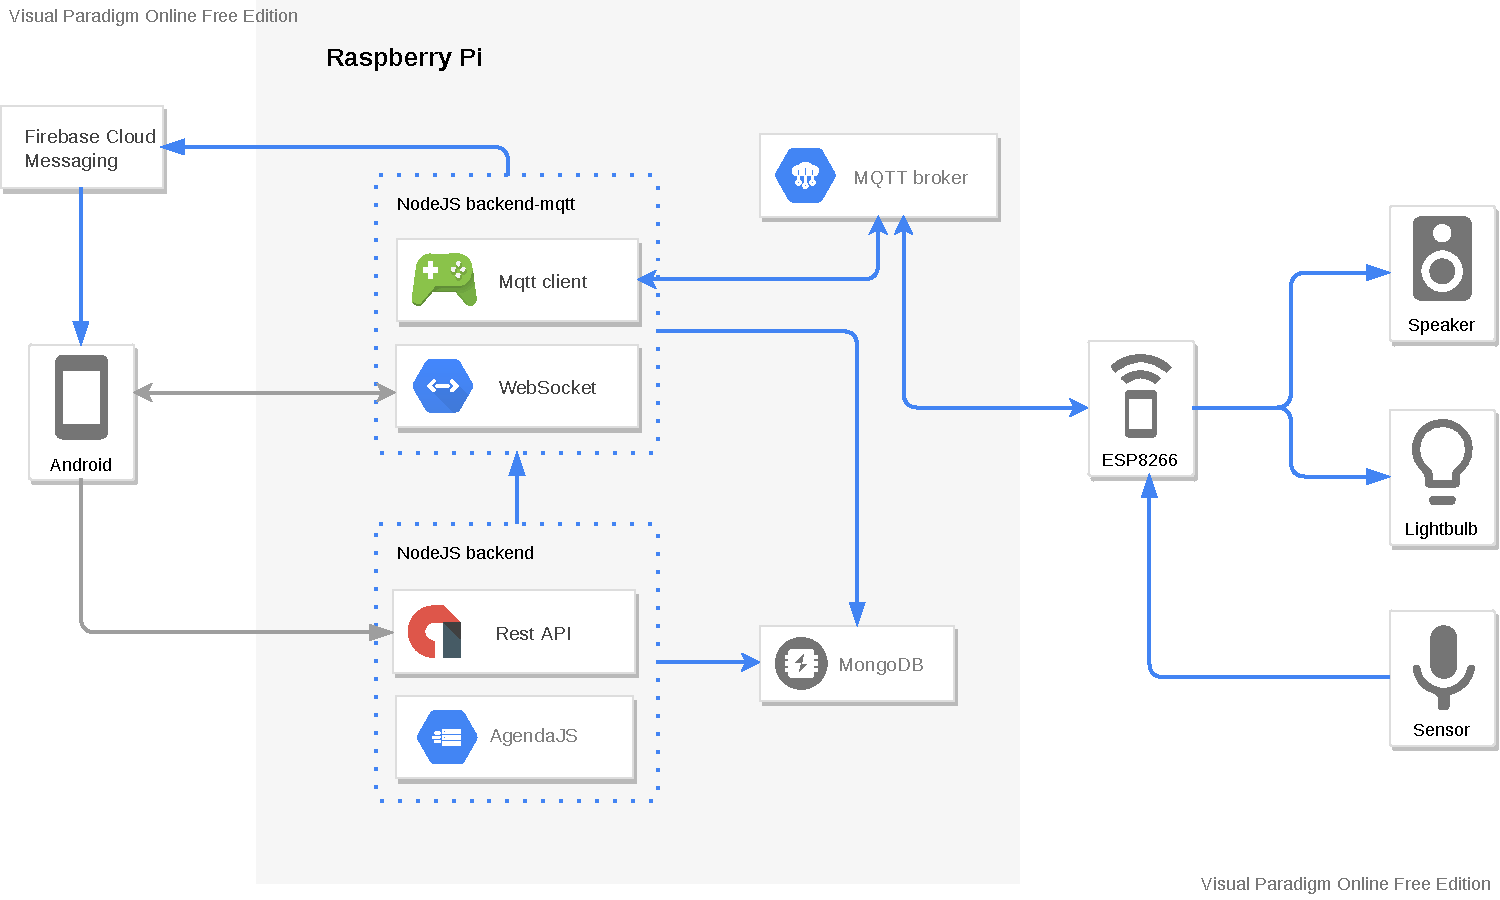
\includegraphics[width=\textwidth]{img/architecture.pdf}
    \caption{Architektura}
\end{figure}

\subsection{Architektura}
Systém implementuje relaxovanou \itshape{Třívrstvou architekturu} obohacenou o \itshape{Publish subscribe pattern}. Základní myšlenkou Třívrstvé architektury je oddělení zodpovědnosti do tří komponenty/vrstev, kde každá komponenta by měla být zodpovědá za určitou čínnost a nepřesahovat svým rozsahem do zodpovědnosti jiné.
\begin{itemize}
    \item Controller (řadič) - prostředník pro komunikaci mezi uživatelem / uživatelským rozhraním a služeb, které systém nabízí
    \item Service (služba) - část systému obsahující aplikační logiku, jejímž úkolem je vykonání jedné věci (např. vytvoření uživatele)
    \item Data access layer (vrstva pro přístup k datům) - vrstva zapouzdřující přístup do databáze, která vytváří dle požadavků příslušné dotazy a výsledky mapuje na objekty
\end{itemize}
\itshape{Publish subscribe pattern} přidává k této architektuře navíc asynchroní zpracování událostí. Toto řešení je velmi užitečné v případě, pokud potřebuje navázat nějaké akce (nejčastěji volání třetí strany např. kvůli analytickým údajům). Například pokud vytvoříme Controller pro registraci uživatele, tak od něj očekáváme, že v vytvoří uživatele a to je vše. Jsou ale situace kdy potřebujeme navázat další akce, které nemají žádnou přímou spojitost s danou odpovědností (např. zalogování do google Analytics nebo odeslání emailu). Přidáním této akce přímo do kontrolleru bychom porušili Princip jedné odpovědnosti (Single-responsibility principle), který říká že každý objekt (v tomto případě kontroler) by měl vykonávat pouze činnost, která se od ní očekává. V tuto chvíli se hodí  \itshape{Publish subscribe pattern}, který umožní v kontroleru vyslání (emit) události, že byl registrován uživatel a veškeré nesouvysející akce se obslouží v obsluze dané události v jiné části systému. Díky tomu nedojde k porušení Principu jedná odpovědnosti a kód kontroleru dělá přesně to, co se od něj očekává a nic víc.

Servrová část je rozdělena na dva separátní procesy kvůli zvýšení odolnosti, aby v případě pádu jedné z části buď fungovalo uživatelské rozhraní nebo část obsluhující komunikaci se zařízeními.
\begin{itemize}
    \item Backend - dává k dispozici RESTful rozhraní pro kompletní ovládání Platformy, dále vykonává naplánová akce jako odesílání emailů
    \item Backend-mqtt - interaguje se zařízeními přes MQTT broker a odesílá real-time změny na frontend
\end{itemize}

\subsection{Databáze}
Pro ukládání dat byla vybrána databáze MongoDB v kombinaci s knihovnou Mongoose. MongoDB je OpenSource dokumentová NoSQL databáze umožňující horizontální škálování. Oproti klasické SQL databázi používá dynamické schéma, díky kterému lze aplikaci mnohem dynamičtěji vyvíjet na rozdíl od SQL databází, kde i malá změna tabulkového schéma v mnoha případech znamená velmi komplikovanou migraci dat. MongoDB používá pro uchovávání dokumentů podobný JSONu (MongoDB nazývá formát BSON), což se velmi snadno kombinuje s jazykem JavaScript, který JSON používá pro nativní objekty.

\paragraph{Mongoose} je knihovna pro NodeJS, která vytváří nad MongoDB objektovou abstrakci a spoustu dalších užitečných funkcí jako validace a type cast. Základním prvkem je definování schéma pro jednotlivé dokumenty, což může vypadat jako návrat do striktního schématu u SQL databází, ale zde je schéma definované pouze na úrovni Mongoose, tedy mnohem flexibilnější a méně restriktivní. MongoDB sice nabízí oficiální knihovnu pro přístup do databáze, ale preferuji Mongoose, protože díky definici schémat mám obecně větší kontrolu nad daty, která se dostanou do databáze. Implementace definuje tyto schémata:
\begin{itemize}
    \item Device - zařízení
    \item Thing - věc zařízení
    \item Notify - seznam notifikačních pravidel pro jednu věc
    \item History - seznam změn stavů věci v čase
    \item User - uživatel
\end{itemize}

\subsection{Souborová struktura}
Oba procesy jsou rozděleny do separátních balíčku \uv{backend} a \uv{backend-mqtt}, které na sobě nejsou nijak závisle a pro sdílení společných částí kódu, primárně databázových modelů, je využíván balíček \uv{common}. Následující souborová struktura pro oba procesy vychází ze článku \href{https://dev.to/santypk4/bulletproof-node-js-project-architecture-4epf}{Bulletproof node.js project architecture}, která se mi velmi osvědčila v osobních projektech.
\dirtree{%
    .1 packages.
    .2 backend\DTcomment{Obsluha RESTful rozhraní a úkolů}.
    .3 src.
    .4 api\DTcomment{zdrojové kódy pro jednotlivé endpointy}.
    .5 device.
    .5 discovery.
    .5 user.
    .4 jobs\DTcomment{definice úkolů pro AgendaJS}.
    .4 loaders\DTcomment{rozdělený startovací proces do modulů}.
    .4 middleware\DTcomment{definice vlastních middleware}.
    .4 services\DTcomment{zdrojové kódy služeb}.
    .4 subscribers\DTcomment{obsluha akcí na asynchroní události}.
    .2 backend-mqtt\DTcomment{Oblsuha MQTT a Socket.IO}.
    .3 src.
    .4 api.
    .5 auth\DTcomment{endpoint pro RabbitMQ autentifikaci}.
    .5 actions\DTcomment{endpoint pro interní komunikaci s Backend}.
    .4 services\DTcomment{zdrojové kódy služeb}.
    .5 firebase\DTcomment{odesílání notifikací}.
    .5 mqtt\DTcomment{napojení na MQTT broker a obsluhu zařízení}.
    .5 websocket\DTcomment{real-time komunikace pomocí Socket.IO}.
    .4 subscribers\DTcomment{definice akcí na asynchroní události}.
    .2 common\DTcomment{Obsahuje sdílené části kódu}.
    .3 src.
    .4 config\DTcomment{konfigurace načtená z promněných prostředí}.
    .4 models\DTcomment{definice mongoose schémat a typů}.
    .4 utils.
}


\subsection{Proces Backend}
Tento proces implementuje webový server nabízející RESTful rozhraní pro vytváření, editaci a mazání všech entit Platformy (uživatel, zařízení). Používá se zde formát dat JSON (JavaScript Object Notation). Dále implementuje odesílání emailů.

\subsubsection{Popis rozhraní}
Všechny endpointy, až na přihlášení a registraci uživatele, vyžadují autentizační token v hlavičce požadavku. Odpověď se potom liší podle oprávnění daného uživatele.
\begin{itemize}
    \item POST /user - vytvoří nového uživatele
    \item GET /device - vrací seznam zařízení
    \item DELETE /device/:deviceId - odstraní dané zařízení
    \item PATCH /device/:deviceId - aktualizuje zařízení
    \item GET /device/:deviceId/thing/:thingId/history?from=\&to - vrací historická data pro specifikovanou věc, parametry from a to specifikují časový rozsah
    \item PUT /device/:deviceId/thing/:thingId/notify - aktualizuje notifikace pro specifikovanou věc
    \item PATCH /device/:deviceId/thing/:thingId - aktualizuje state pro specifickoou věc
\end{itemize}
Více v dokumentaci zdrojového kódu.

Server na požadavky odpovídá následujícími HTTP kódy:
\begin{itemize}
    \item 200 - v pořádku, součásti těla odpovědi jsou data
    \item 204 - v pořádku, tělo odpovědi je prázdné
    \item 400 - chybný požadavek
    \item 403 - nedostatečné oprávnění
    \item 404 - požadovaný zdroj nebyl nalezen
\end{itemize}


\subsection{Proces Backend-mqtt}
Tento proces implemetuje autentizační rozhraní, které používá MQTT broker pro autentifikaci jednotlivých zařízení a je přihlášen k odběru všech zpráv z MQTT brokeru, na které příslušně reaguje - vytváří nově objevená zařízení, ukládá stav zařízení, změny stavu jejich vlastností a odesílá real-time změny na rozhraní pomocí knihovny Socket.IO. Dále implementuje RESTful rozhraní pro interní komunikaci s procesem Backend, které umožňuje nastavení změnu stavu vlastnosti a inicializaci párování nového zařízení. Toto rozhraní je z důvodu oddělejí odpovědností, kdy tento proces řešeí obsluhu zařízení přes MQTT, zatímco proces Backend komunikaci s uživatelským rozhraním.


\subsection{Bezpečnost}
% helmet - popis útoků které brání, rate limmiter, mongo sanitizer ->  JWT token - výhody rychlosti a místa oproti ukládání cookie/session -> nginx jako proxy - separace konfigurace, snažší pro správu sys adminem -> rabbitMQ a custom backend (+cache pro vyšší výkon)
Platforma zpracovává uživatelská data a proto je nutné tyto data chránit (s ohledem na soukromý uživatelů a i z pohledu zákona). Následující text pojednává o implementovaných bezpečnostních mechanizmů.

% TODO OWASP citace https://cheatsheetseries.owasp.org/cheatsheets/Nodejs_Security_Cheat_Sheet.html
RESTful rozhraní je přímo dostupné z internetu a proto je velice důleží ho správně zabezpečit proti zneužití. Proti velkému množství útoků se lze bránit správným nastavením HTTP hlaviček. Toto sice nechrání před přímými útoky, protože útočník může hlavičky ignorovat, ale chrání uživatele tak, že informují jejich prohlížeč o povoleném chování stránky např. odkud je bezpečné stahovat kód. Tímto způsobem lze primárně předejít útokům typu \itshape{Cross-site scripting} (vložení/podstrčení cizího JavaScript kódu do stránky) a jiným druhům \itshape{Cross-site infections} (vkládání html, stylů a jiných objektů) a \itshape{Clickjacking} (překrývání klikacích prvků jinými s úmyslem propagace kliknutí na prvek, který chce útočník). Pro nastavní hlaviček jsem využil middleware \uv{helmet}, který je doporučený projektem OWASP (Open Web Application Project), který se přímo zabývá bezpečností webových aplikací. Pro ochranu přihlášení před útokem typu \itshape{Brute-force} (hrubou silou) jsem použil middleware \uv{express-rate-limit}. Prozatím se základním nastavení s omezením počtu pokusů na jednu ip adresu za určitý časový úsek a data si udržuje v paměti. V případě pootřeby je ale velmi snadno rozšiřitelný o využití databáze (např. Redi) a komplexnější omezení (např. limit pokusů pro kombinaci uživatelského jméno a ip adresy).

Pravděpodobně nejznámější typ útoku je \itshape{SQL Injection}. Díky využití NoSQL databáze systém přímo touto zranitelnosti netrpí přímo, ale jejím ekvivalentem v podobě \itshape{NoSQL Injection}. Princip tohoto útoku je velmi jednoduchý. Zranitelnost vychází ze všech uživatelských vstupů, která se používají pro vytváření dotazů do databáze. Při sestavování těchto dotazů lze chytře využít možnost daného dialektu databázového jazyka a kompletně modofikovat jeho význam. Způsob ochrany spočívá v odstranění/nahrzení všech potencionálně zneužitelných znaků v uživatelstkém vstupu. Konkrétně jsem využil middleware \uv{express-mongo-sanitize}, který odstraní ze všech potencionálně zneužitelných míst všechny znaky \uv{\$} a \uv{.}, které lze v případě MongoDB využít právě pro \itshape{NoSQL Injection}.

Do systému mohou přistupovat klienti pod různými uživatelskými účty, která mají různá oprávnění vázaná k určitým zařízením. Proto je nutné zamezit přístup pouze k takovým zdrojům serveru, ke kterým má daný přihlášený uživatal přístup. Jak vlastně server pozná kdo inicioval daný požadavek? V případě nestavového protokolu HTTP, musí iniciátor přiloži ke každému požadavku nějaký token, kterým prokáže svojí totožnost. K tomuto účelu se nejčastěni využívaly dlouhé náhodné unikátní identifikátory, které byly uloženy v databázi u daného uživatele. Toto řešení ale vyžadovalo dotaz do databáze při každém požadavku pro ověření identity, což zbytečně zvyšuje zátěž na server. Proto se vytvořil standart využívající asymetrickou kryptografii JWT (JSON Web Token, RFC 7519), který umožňuje při přihlášení klientovi odeslat řetězec obsahující informace (např. id, jméno, příjmení, úrověň oprávnění) a asymetrická kryptografie zaručuje, že nelze tyto informace modifikovat bez poškození integrity. Díky tomu odpadá nutnost pokaždé se dotazovat do databáze, protože stačí ověřit integritu tokenu. Tento postup má samozřejmně, ale i své negativní vlastnoti, kterými se zde však nebudeme zabývat.

%https://news.netcraft.com/archives/category/web-server-survey/
Věřím, že využití HTTPS (HTTP spolu se šifrováním SSL nebo TLS) je dnes samozřejmností v případě, že se na stránce zadávají jakékoli údaje. NodeJS přímo podporuje šifrované HTTP, ale správa certifikátu i nastavení není úplně přímočaré. Proto jsem NodeJS použil jako HTTP server s představeným proxy serverem Nginx, který s klienty již komunikuje pomocí zabezpečeného spojení. Nginx je široce podporován různými nástroji pro správu webů mimo jiné nástrojem \uv{Certbot}, který umožňuje automatické získání bezplatného certifikátu nutného pro provoz HTTPS. Lze velmi snadno konfigurovat a nabízí pokročilé funkce jako \itshape{load balancing}.

Veškerá komunikace mezi koncovými zařízeními a Platformou probíhá přes protokol MQTT a proto zabezpečení tohoto kanál je nezbytné. Není žádoucí aby třetí strana mohla posílat požadavky pro změnu stavu zařízením, i odposlouchávání zpráv je bezpečnostní riziko (z odposlechu pohybovích čidel lze zjistit zda je někdo doma, zlatý důl pro zloděje). Šifrování MQTT dokáže zajistit využití protokolu nižší vrstvy TLS (označováno jako mqtts nebo mqtt over tls). Toto řešení zamezí odposlechnutí komunikace mezi Brokerem a zařízením. Většina existujících řešení pro domácnost další bezpečností prvky neimplementují a následkem toho sice nelze odposlechnout komunikace, ale lze se jednoduše přihlást k Brokeru k odběru všech zpráv. Já však považuji toto řešení jako nedostatečné a proto implementuji systém pro autentizaci (ověření identity) i autorizaci (kontrola oprávnění pro přístup k danému zdroji). MQTT specifikace umožňuje přihlášení pomocí uživ. jména a hesla nebo certifikátu. Vzhledem k omezenému výpočetnímu výkoun ESP8266 jsem nucen využít kombinaci jména a hesla, protože rozumný výpočet asymetrických šifer je za hranicí jeho možností. Jako MQTT Broker využívám RabbitMQ, který podporuje definici vlastního backendu pro kontrolu oprávnění přes RESTful rozhraní. Toto řešení mi umožňuje kontrolovat přihlášení jednotlivých zařízení a i následně jednotlivé požadavky k publikaci a odběru zpráv. Součástí dat, které předává RabbitMQ autentizačnímu serveru je i název tématu do kterého chce zařízení zapisovat nebo z něho číst a můžu, tak přesně specifikovat jestli to danému zařízení umožní či nikoliv.

\subsection{Validace}
\label{BE:Validace}
% Vlastní framework, interaktivní validac na FE -> best UX, descriptory
Webové aplikace se stávají stále více komplexní se složitější datovou strukturou. Z pohledu systému je pro nás důležité validovat veškerá data, která přijdou od třetí strany před tím, než s nimi začneme pracovat, protože se nemůžeme pouze spoléhat, že nám je někdo poslal ve správném formátu, v horším případě útočník bude záměrně posílat chybná data s nějakým postraním úmyslem. Z pohledu uživatele, je pro něj důležité, aby formulář byl intuitivní a na případné chybně zadané hodnoty byl ihned upozorněn - z vlastní zkušenosti vím, že není nic horšího než vyplnit dlouhý formulář, který se zdá naprosto validní, stisknout tlačítko odeslat a následně vidět nic neříkající hlášku \uv{Nevalidní formulář} bez jakýhkoli upřesňujícíh informací.

%http://sumitshresthatech.blogspot.com/2012/03/field-and-field-descriptor-pattern.html
Využití stejného programovaícho jazyka jak na backendu, tak frontendu mi umožňuje využít stejný způsob validace dat na obou stranách, který poskytne uživateli okamžitou odezvu bez nutnosti duplikace validační logiky. Implementoval jsem si proto vlastní framework, který je založen na vzoru \uv{Field and Descriptor Field}. Podle tohoto vzoru vstupují do systému dva separátní vstupy. Field obsahuje reálnou hodnotu pole a Deskriptor popisuje správný formát hodnoty pole. Systém při validaci určitého hodnoty si nejprve načte příslušný deskriptor a následně aplikuje validační logiku dle konfigurace v deskriptoru.

Pomocí deskriptorů se definují struktury dat celých formulářů. Každý RESTful endpoint konzumuje v tělě požadavku formulář, který je předem systémem zvalidován (pomocí middlewaru). Výstupem validace je seznam všech polí, která nejsou validní a chybové hlášky obsahující přesný popis proč validace selhala.

\subsubsection{Field Deskriptor}
Deskriptor se definuje pro každé formulářové pole, společně tvořící deskriptor pro celý jeden formulář. Datovou struktura reprezentující formulář lze libovolně zanořovat a struktura odpovídá 1:1 struktuře držící samotná formulářová data. Ukázka deskriptoru pro formulář obsahující jedno pole:

\begin{verbatim}
{
    FORM_NAME: {
        userName: {
            // sebereflektivní cesta k deskriptoru
            deepPath: "FORM_NAME.userName",        
            label: "Název který se zobrazí u pole v UI",
            // pokud vrátí false, tak required bude ingorováno
            when: (formData) => formData.selected === "user", 
            // povinost vyplnění pole 
            required: true/false,
            // seznam validací, kterými se má validovat hodnota
            validations: [
                validationFactory('isString', {min: 3, max: 10})
            ],   
        }
    }
}
\end{verbatim}


\subsection{MQTT schéma}
% popis Homie komunikace + vlastní modifikace, ukázka na diagramu
První prototyp jsem založil na vlastní struktuře témat na MQTT protokolu, na kterém zařízení ohlašovali v jakém stavu se nachází a naslouchaly pro případně požadavky na změnu. Uživatel při vytváření zařízení musel nadefinovat veškeré jeho vlastnosti pomocí poměrně rozshálích formulářů, následně se vygeneroval api klíč a ten musel zadat do zařízení pro jeho úspěšné přihlášení k platformě. Toto řešení se ukázalo jako nešťastné, protože uživatel pro přidání zařízení musel mít rozsáhlé znalosti dané problematiky a tento proces byl velice časově náročný. Proto jsem se rozhodl, že místo toho aby uživatel definoval ručně každé zařízení, tak zavedu automatickou detekci (auto discovery) nových zařízení, které budou sama propagovat Platformě jaké věci a vlastnosti podporují.

Po mnohých experimentech jsem nakonec své řešení založil na konvenci \uv{Homie} specifikující strukturu MQTT témat pro automatickou detekci, konfiguraci a používání zařízení. Tento základ jsem obohotil mimo jiné o výmněnu párovacího klíče a z důvodu, že konvence počítá s globálním unikátním identifikátorem pro každé zařízení, tak jsem přidal navíc unikátní prefix pro MQTT téma, které označuji jako \uv{realm} - tento prefix je unikátní pro každého uživatele a všechny jeho zařízení komunikují v tomto realmu. Toto mi umožňilo omezit unikátnost identifikátoru z globálního na úroveň uživatele. Moje řešení neimplementuje kompletní konveci, ale pouze následující čast.

Základem \uv{Homie} konvence je, že každé zařízení obsahuje uzly (věci) a ty mají vlasnosti. Přiklad - zařízení auto má uzel motor, které má vlastnosti teplotu a tlak. Každé zařízení komunikuje v tématu obsahující nějaký prefix a v další úrovní id daného zařízení (ukázka \uv{homie/esp-1919/}). Homie specifiku základní atributy tématu, které se používají pro konfiguraci a začínají symbolem \uv{\$}:
\begin{itemize}
    \item \$name - člověkem čitelný název.
    \item \$state - v jakém stavu se dané zařízení nachází. Init - zařízení je připojené, ale ještě není plně připraveno. Ready - je připraveno a plně funkční. Disconnected - odpojeno. Lost - ztráta spojení (zařízení je poviné toto zadefinovat jako \hyperlink{LWT}{Last Will Testament}). Alert - zařízení vyžaduje pozornost
    \item \$nodes - seznam id uzlů, které zařízení obsahuje oddělené čárkou.
\end{itemize}

Pro prefix tématu \uv{homie/esp-1919/nodeId} lze odeslat následující atributy:
\begin{itemize}
    \item \$name - člověkem čitelný název uzlu
    \item \$type - typ uzlu
    \item \$properties - seznam id vlastností, které daný uzel obsahuje oddělené čárkou
\end{itemize}

Pro prefix tématu \uv{homie/esp-1919/nodeId/propertyId} lze odeslat následující atributy:
\begin{itemize}
    \item \$name - člověkem čitelný název vlastnosti
    \item \$datatype - datový typ hodnoty vlastnosti (string, float, integer, boolean, enum).
    \item \$unit - jednotka hodnoty vlastnosti. [volitelný]
    \item \$format - specifikace omezení pro daný datový typ. Pro float, integer lze uvést rozsah hodnot ve formátu minimální a maximální hodnota oddělená dvojtečkou (např. \uv{10:20} pro rozsah 10-20). Pro enum se specifikuje výčet možných hodnot oddělených čárkou (např. \uv{red,blue,orange}) [volitelný]
    \item \$settable - informace zda lze hodnotu vlastnosti nastavit (true, false). [volitelný, výchozí false]
\end{itemize}


%\begin{verbatim}
%prefix/deviceId/$name   -> Název zařízení
%prefix/deviceId/$nodes  -> seznam nodeId
%prefix/deviceId/nodeId/$name    -> Název uzlu
%prefix/deviceId/nodeId/$type    ->
%prefix/deviceId/nodeId/$properties
%    -> seznam propertyId
%prefix/deviceId/nodeId/propertyId -> Aktuální hodnota
%prefix/deviceId/nodeId/propertyId/$name -> Název
%prefix/deviceId/nodeId/propertyId/$datatype -> Datový typ
%prefix/deviceId/nodeId/propertyId/$unit -> Jednotka hodnoty
%prefix/deviceId/nodeId/propertyId/$settable
%    -> Lze/nelze nastavit vlastnost
%prefix/deviceId/nodeId/propertyId/set
%    -> Zařízení naslouchá pro změny pokud je settable
%\end{verbatim}

\subsubsection{Upravená specifikace}
Rozdíl v mém řešení oproti \uv{Homie} konvenci primárně spočívá v použítí dvou rozdílným prefixů témat v závislosti jestli zařízení již bylo spárováno (uživatel si dané zařízení přidal) či nikoliv. Při prvním připojení se zařízení ohlásí v prefixu \uv{prefix/} následovaný identifikátorem zařízení stejně jako v případě homie konvence. Oznámí svůj status, název a všechny své schopnosti (věci a vlastnosti). Toto téma je veřejně přístupné pro všechny zařízení, která se k MQTT brokeru přihlásí uživatelským jménem shodujícím se s identifikátorem zařízení narozdíl od druhého prefixu \uv{v2/{realm}}, který je přístupný pouze zařízení, který s přihlásí pomocí platného api klíče s přístupem do daného realmu. Přidané atributy:
\begin{itemize}
    \item \$realm - do kterého realmu zařízení chce patřit (uživ. jméno uživatele)
    \item \$config/apiKey/set - tento atribut využívá Platforma pro odeslání api klíče. Zařízení je zodpovědně za přihlášení odběřu daného tématu.
\end{itemize}

Přidán atribut pro téma definující vlastnost:
\begin{itemize}
    \item \$class - do jaké třídy hodnota vlastnosti patří, možnosti: humidity, temperature, voltage, pressure. Tato hodnota ovlivňuje pouze uživatelské rozhraní, specificky jaká ikonka se u hodnoty zobrazí. [volitelné]
\end{itemize}


Následuje ukázka komunikace pro automatickou detekci zařízení umožňující zapnutí/vypnutí světla, měření teploty s identifikátorem \uv{light} a hlásící se k uživateli s uživ. jménem \uv{pepa}:
\begin{verbatim}
prefix/light/$status   -> init
prefix/light/$name   -> Světlo
prefix/light/$nodes  -> sensor,switch
prefix/light/$realm  -> pepa
prefix/light/sensor/$name    -> Senzor
prefix/light/sensor/$type    -> sensor
prefix/light/sensor/$properties -> temperature
prefix/light/sensor/temperature/$name -> Teplota
prefix/light/sensor/temperature/$datatype -> float
prefix/light/sensor/temperature/$unit -> °C
prefix/light/sensor/temperature/$class -> temperature
prefix/light/switch/$name   -> Lustr
prefix/light/switch/$type   -> switch
prefix/light/$status    -> ready
\end{verbatim}

Pokud se detekované zařízení nachází ve stavu \uv{ready}, tak je zobrazeno příslušnému uživateli pro přidání. Pokud si ho uživatel přidá, tak Platforma odešle api klíč danému zařízení, který jeho přijetí potvrdí, klíč si uloží a následně se přepne do prefixu témat \uv{v2/{realm}/}. Pokračování ukázky:

\begin{verbatim}
prefix/light/$apiKey/set
    -> XXXXXXXXXXXXXXXX (odesláno Platformou)

prefix/light/$status    -> paired
prefix/light/$status    -> disconnected
v2/pepa/light/$status   -> ready

v2/pepa/light/sensor/temperature   -> 20.05
v2/pepa/light/switch/power         -> on
\end{verbatim}

\begin{figure}[htbp]
    \centering
    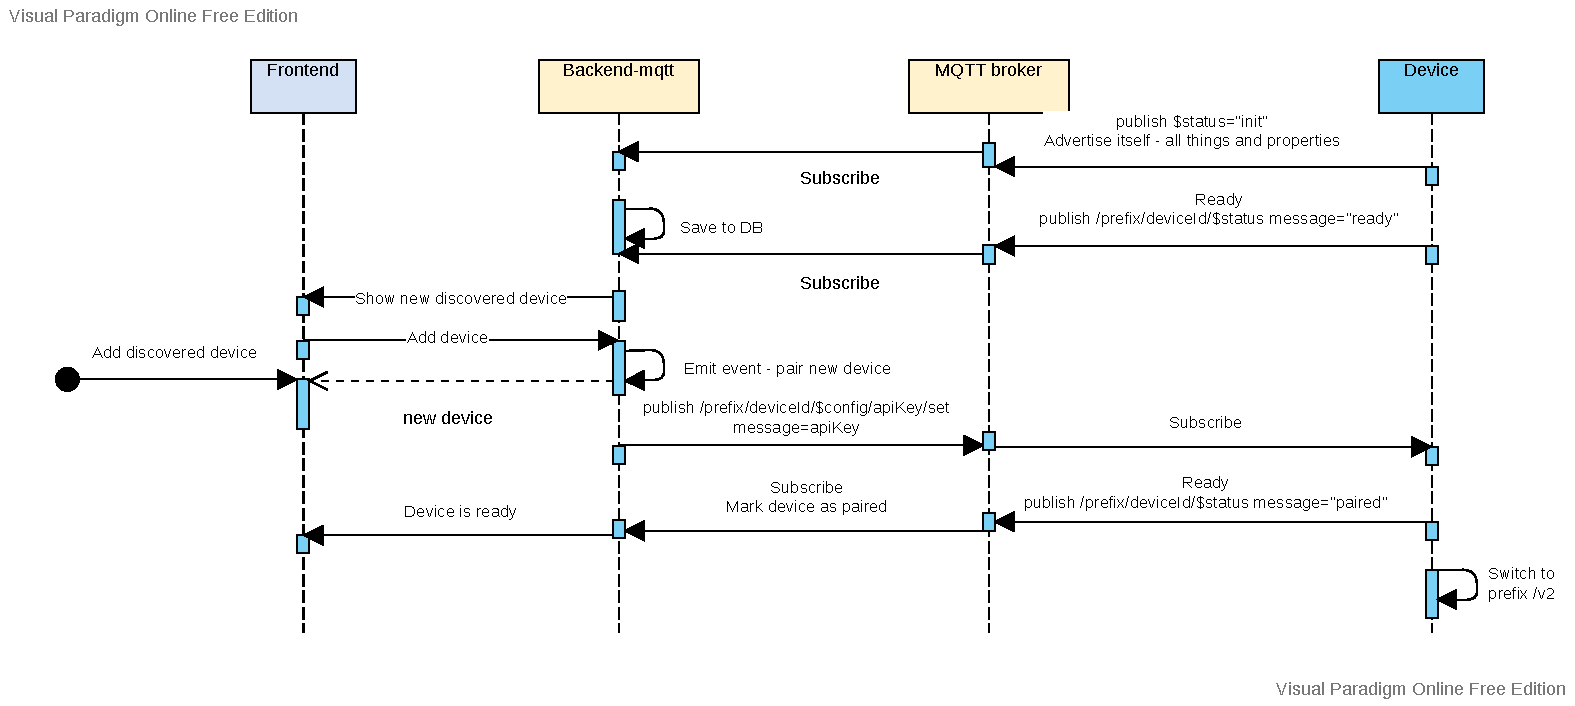
\includegraphics[width=\textwidth]{img/pairing_communication.pdf}
    \caption{Proces přidání zařízení}
\end{figure}

\section{Uživatelské rozhraní}
% Popis PWA, SPA, struktura složek, webSocket, no cookie (local storage)
Tato sekce se zabývá architekturou a implementací uživatelského rozhraní formou webov stránky. Implementace je rozdělena do dvou balíčků:
\begin{itemize}
    \item Framework-ui - obsahuje komplexní řešení pro validace formulářů včetně integrace s Redux (napojení na state, definice akcí a reducerů), implementuje znovu použitelné React komponenty, včetně komponenty řešící přímého napojení formulářového pole na state a obsluhu jeho validací (FieldConnector). Dále jazykovou lokalizaci pro systémové hlášky a nádstavbu nad fetch (api pro odesílání HTTP požadavků), která řeší zobrazení chybových hlášek a definuje flexibilnější rozhraní.
    \item Frontend - implementace samotné aplikace
\end{itemize}

\subsection{Frontend}
Uživatelské rozhraní je realizováno jako SPA - průchod celou aplikací je plynulý a nikdy nedochází k přenačítání celé stránky, ale pouze k překresleních potřebných částí. Toto řešení zlepšuje uživatelský zážitek, protože stránka zůstává pořád plně aktivní a při čekání na vyřižení požadavku uživatel může pokračovat v interakci. Také je zde implementován standard PWA - v podporovaných systémech jako je např. android lze aplikaci tzv. \uv{Přidat na plochu}, potom při otevření vypadá jako nativní aplikace (nemá zobrazený url bar). Statické soubory jsou v cache, díky čemuž je minimalizován datový přenost a stav aplikace je perzistentně ukládán, takže při zavření aplikace a následném otevření je stav plně obnoven a uživatel pokračuje přesně tam kde skončil naposledy.

\subsubsection{State management}%https://redux.js.org/introduction/getting-started
React je postavený na předávání dat mezi jednotlivými komponenty, které tvoří stromovou strukturu, data lze však předávat primárně z vrchu dolů a proto je poměrně složité ze spodní komponenty předat změnu do vrchní. Navíc dnešní aplikace pracují s obrovským množstvím dat, ke kterým potřebují přistupovat různé části aplikace a ideálně transparentní cestou je modifikovat a této modifikaci se musí dozvědět všechny komponenty, pracující s danými daty aby dostali jejich aktuální verzi. Dnes již React obsahuje řešení složitější předávání dat, ale já jsem se rozhodl pro využití komplexní řešení s centrálním úložištěm stavu aplikace v podobě knihovny Redux, které nabízí více funkcí a je odzkoušené časem. Redux je založený na \uv{Observer pattern}. Tento návrhový vzor definuje dvě entity - předplatitel (posluchč) a vydavatel (pozorovaný). V praxi se jednotlivé komponenty se přihlási k odběru určitých dat \uv{předplatí si} a v případě, že někdo chce data modifikovat, tak se stane vydavatelem a řekne co modifikuje a jak vypadají nová data. Redux se zajistí, že všichni předplatitelé dat, kterých se modifikace týka dostanou jejich nejnovější verzi. V Reduxu se používá následující terminologie:
\begin{itemize}
    \item store - centrální úložiště dat (tvz. \uv{Jediný zdroj pravdy})
    \item akce - popisuje k jaké změně dojde
    \item dispatch akce - odeslání určité akce k vykonání
    \item reducer - reaguje na odeslanou akci, obsahuje logiky pro modifikaci dat
\end{itemize}
% TODO show some nice picture of Redux FLOW

% TODO CSS in JS, material-ui
\subsubsection{Vzhled}
V kombinaci s Reactem jsem použil knihovnu Material-ui, která obsahuje velké množství nastylovaných komponent a komplexní řešení pro stylování React komponent. Tuto knihovnu používám již od prvopočátku jejího vzniku a velmi jsem si ji oblíbil primárně kvůli velmi detailní dokumentaci. Obsahuje vestavěné řešení pro \itshape{CSS-in-JS}, které mi jako programátorovi velmi vyhovuje, protože překlenuje spoustu limitací a obskurností přímého použití CSS. Umožňuje mi definovat vzhled ve stejném souboru i jazyce jako samotnou React komponentu, díky tomu nemusí programátor přepínat kontext mezi různými jazyky a může se plně soustředit na vývoj uživatelského rozhraní.

\subsection{Souborová struktura}
\dirtree{%
    .1 packages.
    .2 framework-ui.
    .3 src.
    .4 api\DTcomment{implementace rozhraní pro odesílání požadavků}.
    .4 Components\DTcomment{React komponenty}.
    .4 localization\DTcomment{řešení pro lokalizaci systémových hlášek}.
    .4 privileges\DTcomment{pomocné funkce pro oprávnění a jejich dědičnost}.
    .4 redux\DTcomment{implementace akci a reducerů, primárně pro správu formulářových dat}.
    .4 validations\DTcomment{implementace validací}.
    .2 frontend.
    .3 public.
    .3 src.
    .4 Pages\DTcomment{jednotlivé stránky rozhraní}.
    .4 api\DTcomment{definice RESTful volání}.
    .4 components\DTcomment{sdílené komponenty napříč stránkami}.
    .4 containers\DTcomment{React kontejnery obalující celou aplikaci}.
    .4 firebase\DTcomment{služba pro registraci a obsluhu notifikací}.
    .4 store\DTcomment{inicializace Redux, definice akcí a reducerů}.
    .4 webSocket\DTcomment{služba pro inicializaci Socket.IO}.
}

\subsection{Validace}
Obecný princip fungování validací je popsán v sekci \hyperref[BE:Validace]{Backend}. Na Frontendu se validace používají pro upozornění uživatele na případně chybně zadanou hodnotu. Samootná formulářová data jsou spravována knihovnou redux, stejně jako celý state aplikace. Jejich struktura je shodná s deskriptory formuláře - deepPath se využívá pro získání příslušné hodnoty.

V Reactu je napsaná komponenta \itshape{FielConnector}, které se předá typ formulářového pole (text, email, select atd.) a deepPath, podle které si nalezne příslušný deskriptor z něhož získá potřebné atributy pro vykreslení formulářového políčka label a name. Následně se provolávají validace v následujících případech:
\begin{itemize}
    \item uživatel poprvé zadává hodnotu a vyklikne (událost \uv{onBlur});
    \item uživatel edituje již zadanou hodnotu, potom se validace spouští po každé změně (událost \uv{onChange}).
\end{itemize}

\subsubsection{Rozhraní}
% TODO jaké obrazovky tam jsou, ukázka z rozhraní
Aplikace nabízí jednoduché uživatelské rozhraní s jedním menu pro navigaci mezi jednotlivými stránkami a tlačítko pro přihlášení, které otevře přihlašovací dialog.

Nepřihlášenému uživateli je k dispozici stránka pro registraci obsahující formulář. Po registraci je automaticky přihlášen a má k dispozici stránku pro správu zařízení a stránku pro ovládání a sledování jednotlivých věcí. Správa zařízení je rozdělena na dvě sekce, první obsahuje tabulku s detekovanými zařízeními, které lze přidat na dvě kliknutí. Druhá část obsahuje tabulku se zařízeními, ke kterým má uživatel oprávnění pro zápis, a může editovat jejich informace, měnit oprávnění pro jednotlivé uživatele a nebo je odstranit.

Stránka pro ovládání a sledování zobrazuje widgety pro jednotlivé místnosti seskupené podle budov. Pokud místnost obsahuje nějakou Věc typu senzor, tak aktuální hodnota je zobrazena na tomto widgetu. Po rozkliknutí místnosti jsou rozbrazena všechny věci, která daná místnost obsahuje. S některými Věcmi lze přímo interagovat (přepínač a aktivátor) a u senzoru je zobrazena aktuální hodnota. U typu generic je po rozkliknutí zobrazen dialog rozbrazující aktuální hodnoty vlastností a případně umožňuje interakci. Po rozkliknutí senzoru je zobrazen dialog, ve kterém je vykreslený graf vizualizující průběh hodnoty v čase za posledních 24 hodin.

Přihlášený uživatel má dále k dispozici stránku s možností editace vlastního uživatelskéhoo účtu a tlačítko pro odhlášení.

Pokud má uživatel admninistrátorské oprávnění, tak má navíc k dispozici stránku pro správu uživatelů, ve které je tabulka zobrazující všechny uživatele s možností jejich editace a odstranění.

\section{Knihovna pro ESP8266}
% Platformio, C++, pubsubclient, OTA
Pro čip ESP8266 lze programovat s využitím oficiálního sdk (Espressif SDK) nebo prostředí Arduino, které se těší obrovské oblibě mezi kutily. Rozhodl jsem se tedy využití prostředí Arduino, protože kolem něho existuje obrovská komunita a stovky již předpřipravených knihoven pro různorodé moduly. Díky tomu není potřeba tolik řešit nízkoúrovňové problémy jako např. implementaci protokolu pro komunikace se senzorem teploty ale stačí si stáhnout příslušnou knihovnu a následedně se plně soustřit na aplikační logiku.

Protože mým cílem je vytvoření Platformy, ke které si bude moci kdokoliv připojit vlastní zařízení, tak abych proces pro všechny co nejvíce zjednodušil, vytvořil jsem knihovnu pro přostředí Arduino, která bude řešit veškerou komunikaci s Platformou a nabídne programátorovi přehledná rozhraní pro definici zařízení, jeho věci, vlastností a reakcí na změny.

Knihovna implementuje následující funkce:
\begin{itemize}
    \item Kaptivní portál - vytvoření wifi přístupového bodu, které po připojení např. telefonu zobrazí webovou stránku na které uživatel zadá přístupové údaje k místní wifi síťi, své uživatelské jméno a případně ip adresu instance Platformy (pouze pokud provozuje vlastní).
    \item Připojení k MQTT brokeru - pro připojení je využita knihovna \textit{pubsubclient}
    \item Objevení zařízení - programátor deklarativním způsobem zadefinuje všechny věci a vlastnosti zařízení, knihovna následně všechny tyto funkce ohlásí Platformě
    \item Spárování - po přidání zařízení uživatelem ve webovém rozhraní obdrží zařízení párovací klíč, který se perzistentně uloží
    \item Definice reakcí - ke každé vlastnosti (v případě, že je nastavitelná) může programátor definovat funkci (callback), který se zavolá v případě, že došlo ke změně dané vlastnosti
    \item OTA - možnost tvz. \uv{aktualizace vzduchem} místo nutnosti fyzického připojení k pc. Podporováno je nahrání firmwaru v rámci lokální sítě a zabezpečeno pouze heslem, kvůli malé paměti a nízkému výkonu pro využití ověření pomocí certifikátů.
\end{itemize}

\section{chytrá udírna} % ukážka deklarace vlastností

\subsection{Návrh zapojení} % zapojení HW

\subsection{Výroba} % fotky 